From table \ref{t: affinities}, we see that \ce{CO2} is a viable option to titrate the reaction products. The possible reactions of \ce{CO2} with \ce{Be+} are unknown in literature, but found to be non-reactive in both ground and excited states, while \ce{C+} readily reacts.

\begin{align}
	\ce{Be+ + CO2 & -> no reaction} \nonumber \\
	\ce{C+ + CO2 & -> CO+ + CO} \label{r: C+CO2->CO} \\
	\ce{& -> CO2+ + C} \label{r: C+CO2->CO2} \\
	\ce{CO+ + CO2 & -> CO2+ + CO} \label{r: CO+CO2->CO2}
\end{align}

Testing the purity of the \ce{CO2}, I introduce the \ce{CO2} into the ion chamber with the RGA.

\begin{figure}[H]
	\centering
	\includegraphics[width=0.7\textwidth]{images/C_CO2_rga.png}
	\caption{\label{fig: cco2 rga} RGA showing purity of \ce{CO2} introduced into chamber. Ratios of \ce{CO2} peaks at $m/z = 12, 16, 28$, and $44$ in agreement with table \ref{t: cco2 fractionation}, with no conclusive evidence of contamination by any other gas.}
\end{figure}

\begin{table}[H]
	\centering
	\label{t: cco2 fractionation}
	\begin{tabular}{|l|l| }
	\hline
	m/z & Fraction \\
	\hline
	44 & 0.85 \\
	28 & 0.05 \\
	16 & 0.05 \\
	12 & 0.012 \\
	\hline
	\end{tabular}
	\caption{RGA fractionation of \ce{CO2} as given by http://ytionline.com/technical-information/rga-spectra-data-fragmentation-factor/}
\end{table}

\subsection{\ce{Be+ + CO2}}
Introducing the \ce{CO2} into the ion chamber to react with only laser cooled \ce{Be+}, The TOF only shows that there are trace amounts of \ce{H2O} in the chamber, with no indication of any further loss due to the inclusion of \ce{CO2}.

\begin{figure}[H]
	\label{fig: Be+CO2 TOF}
	\centering
	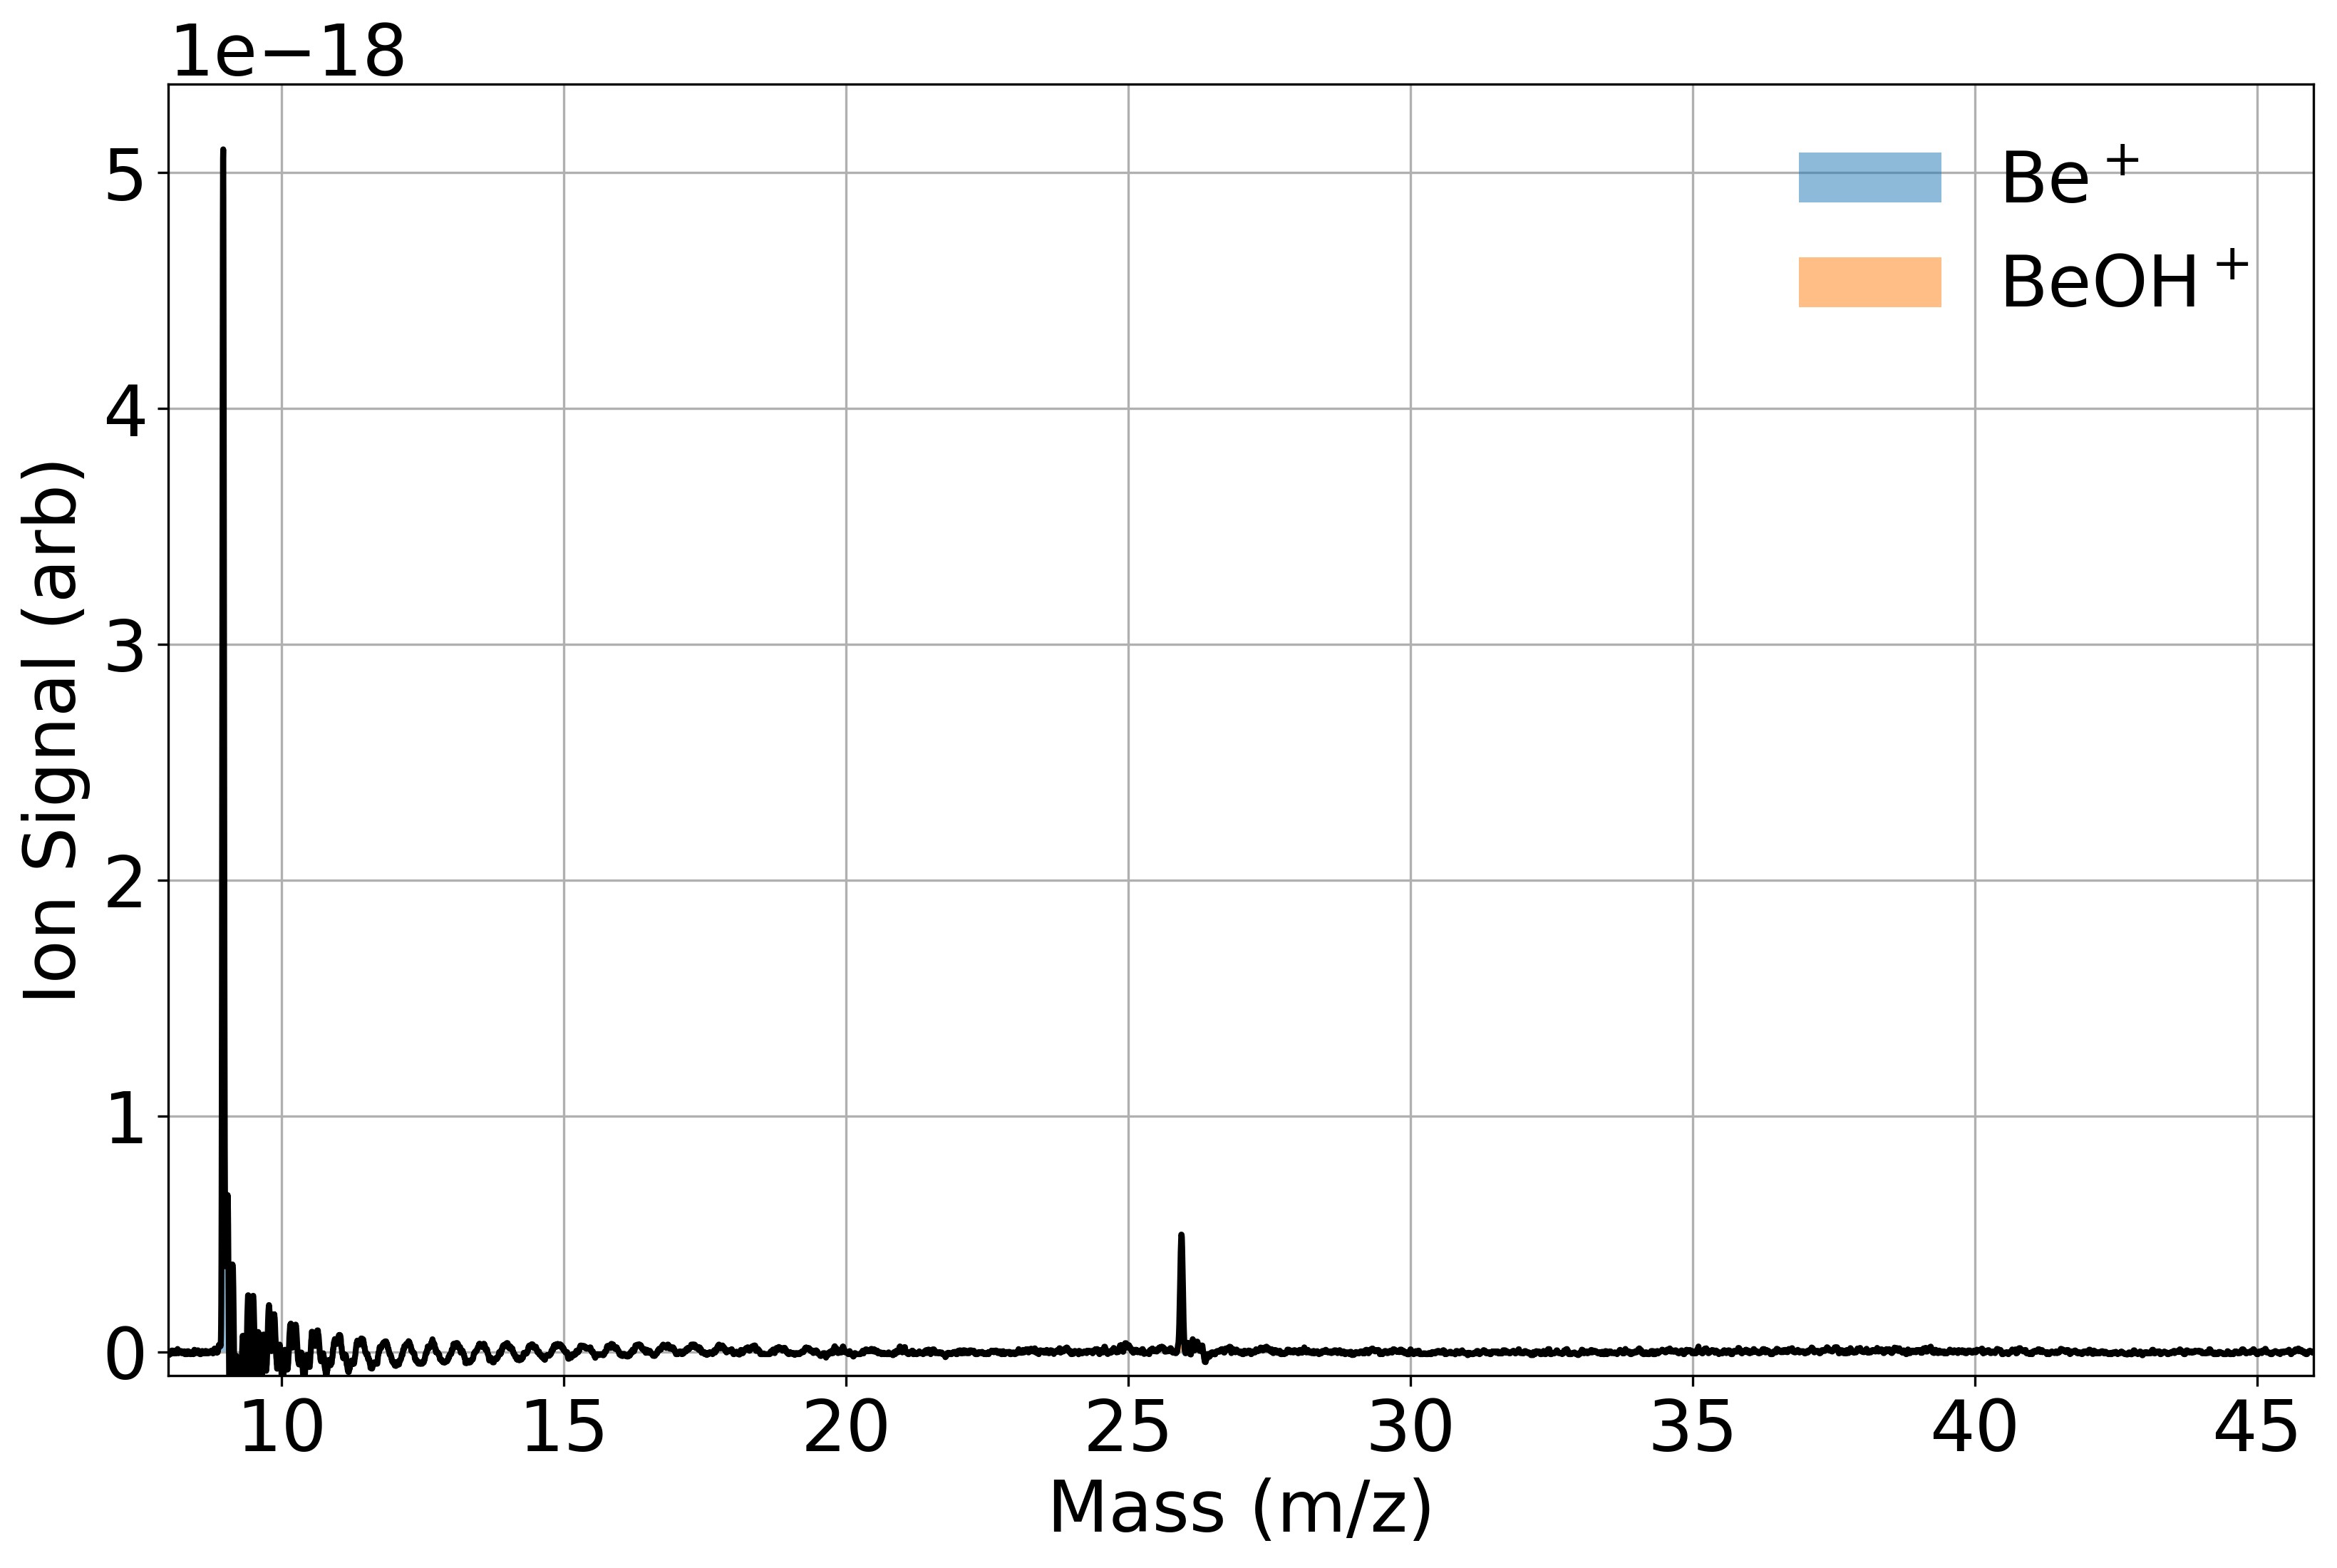
\includegraphics[width=0.8\textwidth]{images/Be_CO2_TOF.png}
	\caption{TOF trace of laser-cooled \ce{Be+} reacting with $\approx 1 \times 10^{-8}$ Torr \ce{CO2} introduced via leak valve for 50 seconds.}
\end{figure}

\begin{figure}[H]
	\label{fig: Be+CO2 traces}
	\centering
	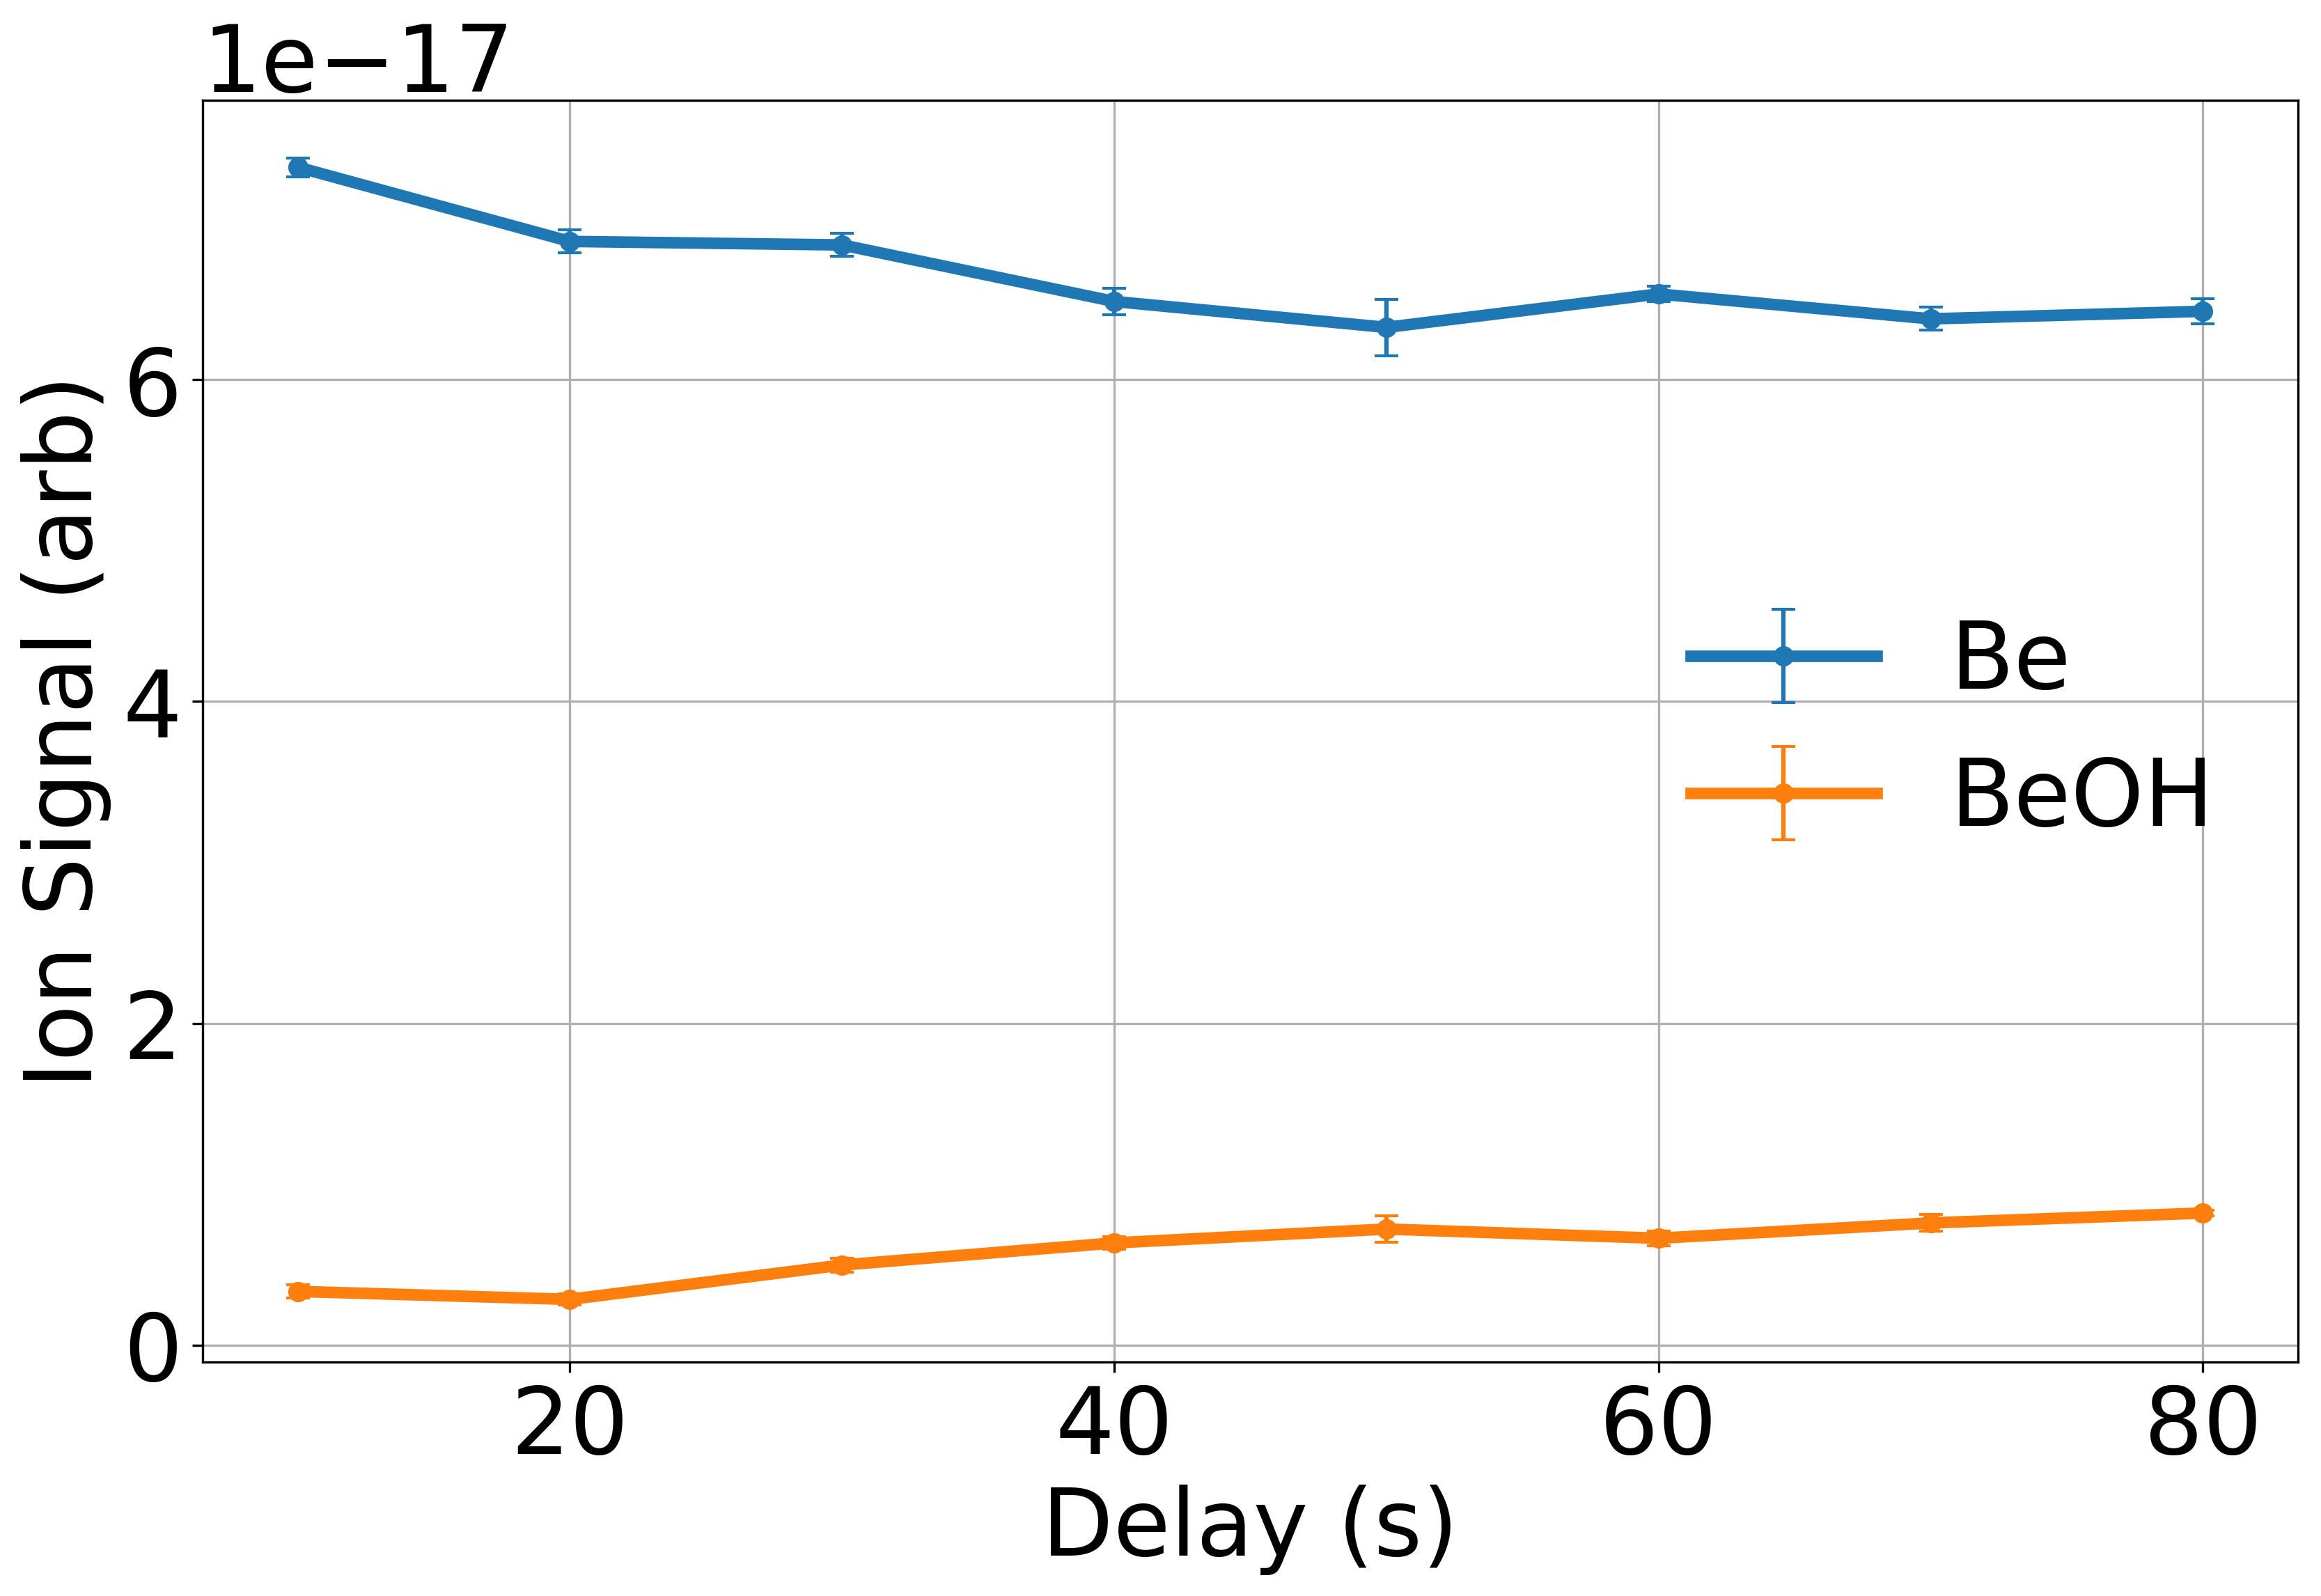
\includegraphics[width=0.8\textwidth]{images/Be_CO2_traces.png}
	\caption{Integrated ion signal of individual TOF traces normalized by \ce{Be+} fluorescence at various \ce{CO2} exposure times.}
\end{figure}

We see that there aren't any reactions happening between \ce{Be+} and \ce{CO2}, while there is a little bit of water in the leak valve, which was baked afterwards. This does indicate that there are also no reactions between \ce{BeOH+} and \ce{CO2}.

\subsection{\ce{C+ + CO2}}
By ablating both \ce{C+} and \ce{Be+} into the trap and introducing \ce{CO2} via the leak valve, we find the expected reactions \ref{r: C+CO2->CO}, \ref{r: C+CO2->CO2}, and \ref{r: CO+CO2->CO2} as well as unexpected peaks appearing at $m/z=15, 29$, and $45$.

\begin{figure}
	\label{fig: C+CO2 TOF}
	\centering
	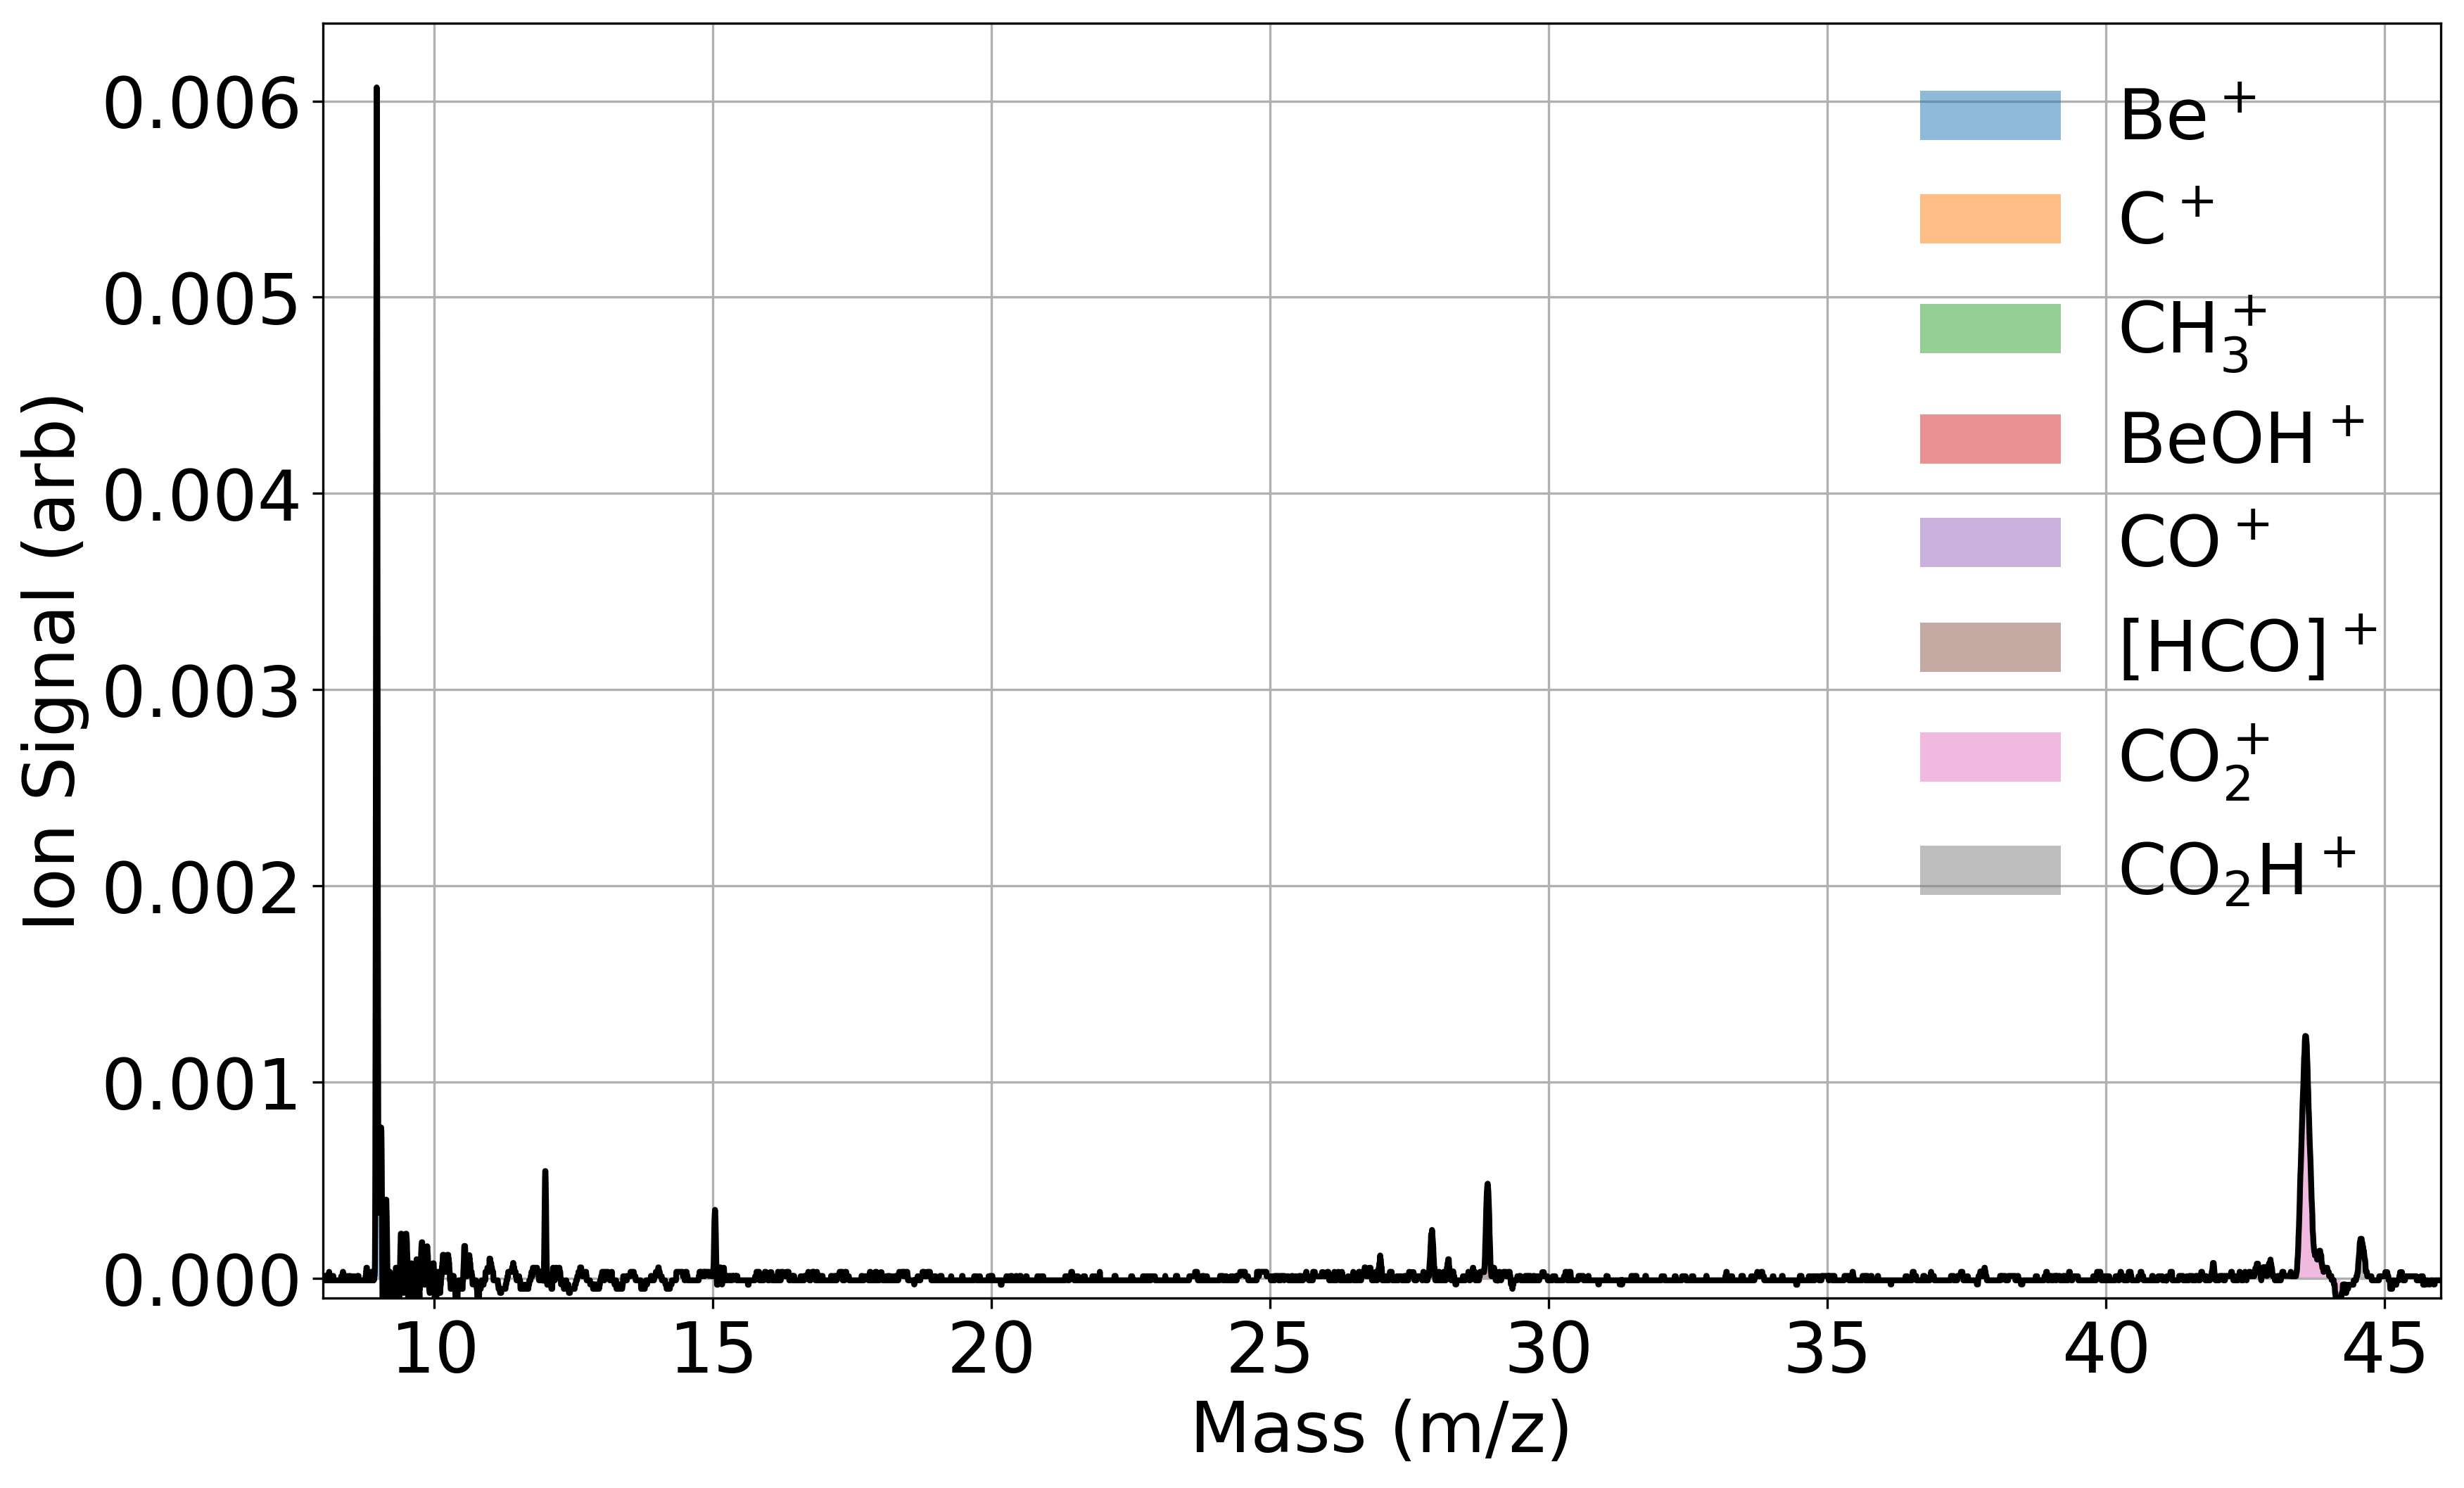
\includegraphics[width=0.8\textwidth]{images/C_CO2_TOF.png}
	\caption{TOF trace of laser-cooled \ce{Be+} and \ce{C+} reacting with $\approx 1 \times 10^{-8}$ Torr \ce{CO2} introduced via leak valve for 40 seconds.}
\end{figure}

\begin{figure}
	\label{fig: C+CO2 traces}
	\centering
	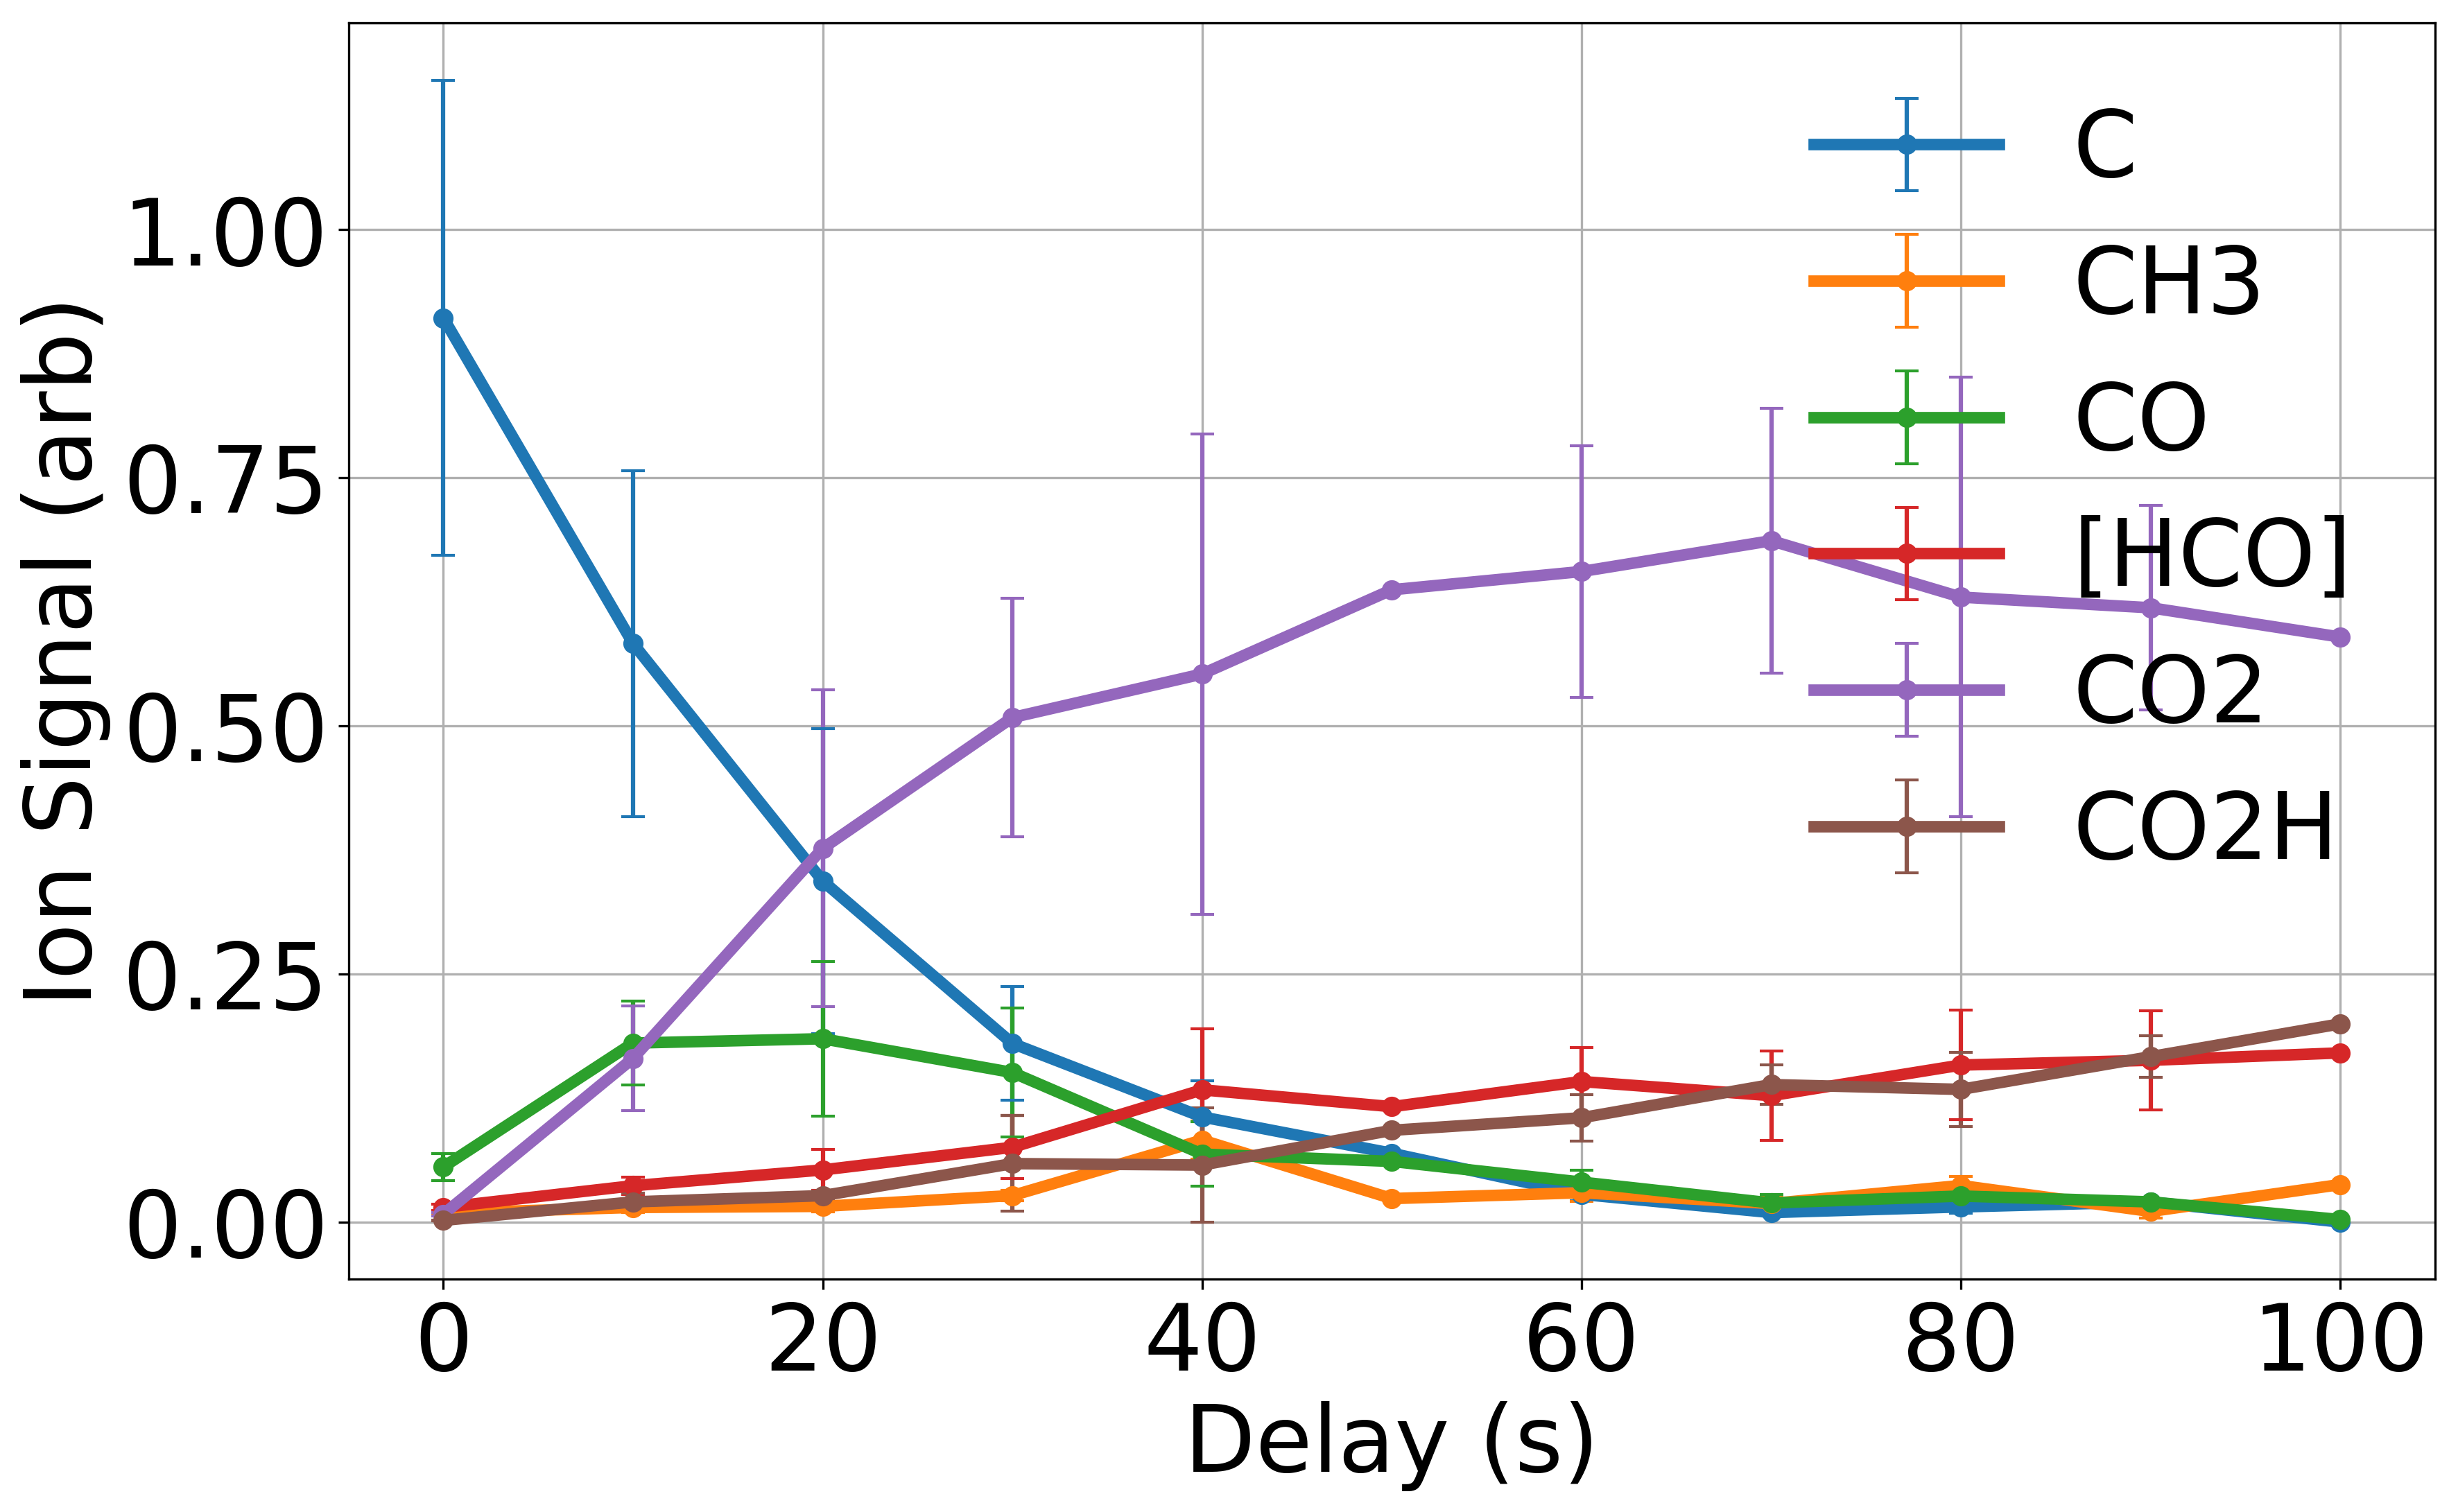
\includegraphics[width=0.8\textwidth]{images/C_CO2_traces.png}
	\caption{Integrated ion signal of individual TOF traces normalized by total ion signal excluding \ce{Be+} at various \ce{CO2} exposure times.}
\end{figure}

Labels in figures \cref{fig: C+CO2 TOF,fig: C+CO2 traces} are of predicted chemicals coinciding with the masses. The initial guess is that there is \ce{H2O} in the leak valve, as we saw it before in the \ce{Be+ + CO2} reaction, but the leak valve region was baked since that data was taken. Similarly, if there was water, we would see a peak at $m/z=26$, coinciding with \ce{BeOH+}, which we do not see, we should also expect to see an abundance of \ce{H3O+} due to reactions between the alleged \ce{[HCO]+} and \ce{CO2H+}, which we also do not see. But, the peak at 45 could possibly be explained by \ce{H2O} in reaction \ref{r: CO2+H2O->CO2H}, while 29 could be due to reactions \ref{r: C+H2O->COH} and \ref{r: C+H2O->HCO}. But there are no reactions with \ce{H2O} for the production of 15.

\begin{align}
	\ce{CO+ + H2O & -> H2O+ + CO} \\
	\ce{CO2+ + H2O & -> CO2H+ + OH} \label{r: CO2+H2O->CO2H} \\
	\ce{CO2H+ + H2O & -> H3O+ + CO2}
\end{align}

I still doubt that the 29 mass is due to \ce{C+} directly reacting with \ce{H2O} because the traces clearly show it increasing despite the depletion of \ce{C+}, indicating it is a second order reaction. It wouldn't be \ce{H2} either, because we would see \ce{BeH+} in the trap, as well as many other peaks associated with \ce{C+ + H2} including 14, 16, and 17.

\subsection{\ce{Be+ + C+ + H2O} with \ce{CO2}}
Water is introduced into the chamber via the CBGB with the cell held at a temperature of 20K. After $(10 \pm 1)$ seconds of exposure, the gate valve is closed and \ce{CO2} is leaked in to react away the formyl isomers such that $\approx 99\%$ are reacted away (determined by the disappearance of \ce{C+}).

\begin{figure}[H]
	\centering
	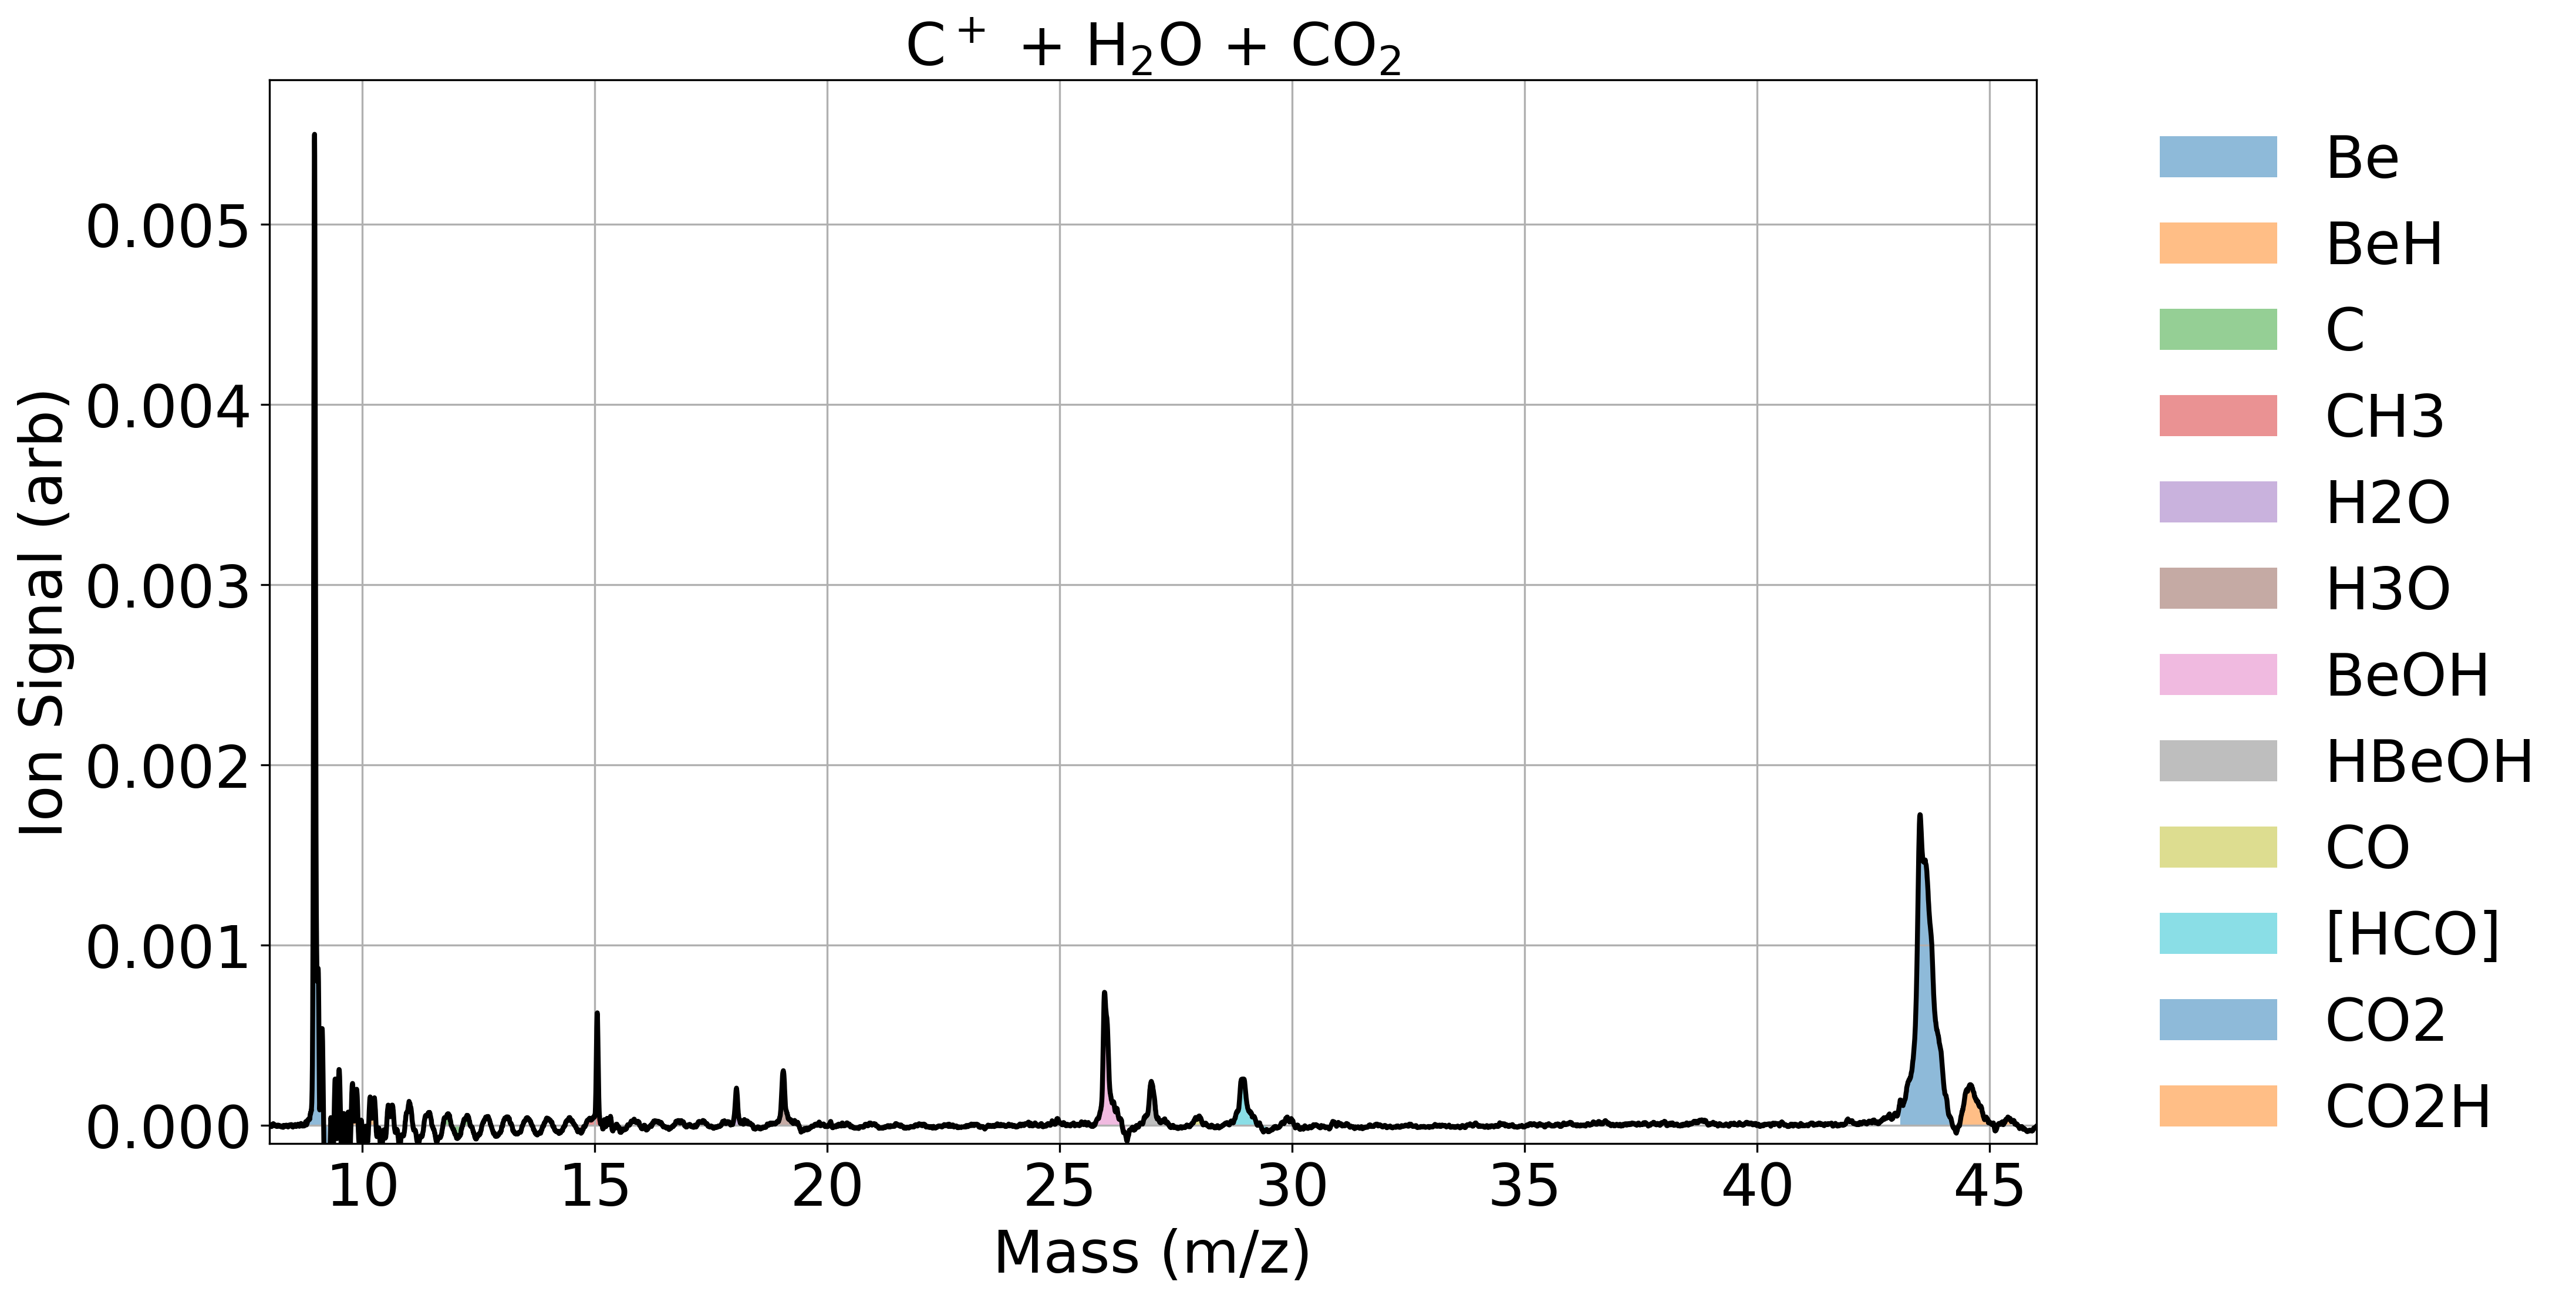
\includegraphics[width=0.9\textwidth]{images/C_H2O_CO2_titration_TOF.png}
	\caption{\ce{C+} and \ce{Be+} loaded into the trap is reacted with \ce{H2O} introduced from the beam. The gate valve is closed after 10 seconds and \ce{CO2} is introduced via leak valve so that the \ce{COH+} is titrated into \ce{CO2H+}.}
\end{figure}

Knowing the anomalous peaks in the previous tests, the peaks of interest are not exclusively the branching ratio between the formyl isomers, where we define $\gamma$ as the fraction of products that produce \ce{COH+}.

Solving the differential equations of the \ce{C+ + H2O} reactions (\cref{r: C+H2O->COH,r: C+H2O->HCO,r: [HCO]+H2O->H3O}, we may derive the equations of the ion reactions:

We define the ratio of the formyl isomers and remaining \ce{C+}

\begin{equation}
	\alpha(t) \equiv \frac{\ce{[HCO](t)}}{\ce{[HCO](t) + C(t)}}
\end{equation}

In the data taken, we introduced the water in the beam for approximately 10s, the fraction of \ce{C+} that has turned into \ce{[HCO]+} is thus $\alpha = 0.37 \pm 0.02$. Considering that after titration with \ce{CO2}, the fraction of the remaining 63\% of \ce{C+} has turned into equal amounts of $m/z=29, 45$ defined as $\beta = 0.17 \pm 0.02$.

\begin{align}
	N_C(0) & = N_0 \\
	N_C(\tau_1) & = (1-\alpha)N_0 \\
	N_{29}(\tau_1) & = \alpha N_0
\end{align}

Where $N_C(t)$ is the amount of \ce{C+} is in the trap after being exposed to either the water beam or \ce{CO2} for time $t$. $\tau_1$ is the amount of time where the ions are exposed to the water beam, where $\alpha$ is the proportion of \ce{C+} that is converted to $m/z=29$, which in our case is 0.37. We then introduce the \ce{CO2} into the system and yield:

\begin{align}
	N_C(\tau_1 + \tau_2) & = 0 \\
	N_{29}(\tau_1 + \tau_2) & = N_{29}(\tau_1)(1-\gamma) + N_C(\tau_1)\beta \\
	& = N_0(\alpha(1-\gamma)+\beta(1-\alpha)) \\
	N_{45}(\tau_1 + \tau_2) & = N_{29}(\tau_1)\gamma + N_C(\tau_1)\beta \\
	& = N_0(\alpha \gamma+\beta(1-\alpha))
\end{align}

In conjuction with the ratio $\eta \equiv \frac{\ce{CO2H+}}{\ce{CO2H+} + \ce{HCO+}} = 0.55 \pm 0.02$

\begin{align}
	\eta & = \frac{N_{45}(\tau_1 + \tau_2)}{N_{29}(\tau_1 + \tau_2) + N_{45}(\tau_1 + \tau_2)}
\end{align}

But we know that there are contributions to both masses of interest due to the inclusion of the \ce{CO2}, thus, we need to solve for $\gamma$:

\begin{align}
	\eta & = \frac{\beta - \alpha \beta + \alpha \gamma}{\alpha + 2\beta - 2\alpha\beta} \\
	\gamma & = \frac{1}{\alpha} (\alpha \eta + \beta(\alpha + 2\eta - 2\alpha \eta - 1)) \label{e: gamma branching ratio}
\end{align}

Using equation \ref{e: gamma branching ratio}, we find at the true branching ratio is scaled from $0.55 \pm 0.03$ to $0.58 \pm 0.05$.
